% TODO: images are on counted
\section{ЗАДАЧІ МАРКЕТИНГОВОЇ РОЗВІДКИ ТА МОДЕЛЮВАННЯ МАРКЕТИНГОВИХ КАНАЛІВ}
% Ми не створюємо канал як такий. Метою роботи є маркетингове прогнозування 
% шляхом моделювання маркетингового каналу.
%
% TODO: можливо, заголовок треба буде змінити
% TODO: додати новий сорець
\subsection{Основні проблемі розробки програмних систем}
\subsubsection{Основні поняття}
% TODO: програмна інженерія
% TODO: програмне забезпечення
% TODO: системна вимога
% TODO: програмний засіб
% TODO: системні вимоги
% TODO: проблемна область  
\subsubsection{Необхідність створення ПС}
\subsubsection{Процес розробки ПЗ}
% TODO: МЖЦ, методології
\subsubsection{Нотація, що використовується}
% TODO: UML, IDEF*

\subsection{Маркетингові інформаційні системи}
% \subsubsection{Необхідність створення МІС}

% \subsubsection{Проблеми МІС}
% \subsubsection{Маркетингова розвідка}
% \subsubsection{Бізнес-ігри}

\subsubsection{Огляд МІС} 
% TODO: додати цю абревіацію до відповідного розділу
% TODO: тупе визначення маркетингу, не в’яжеться взгалалі. Придумати нову структуру.
За визначенням Американської асоціації маркетингу, {\it маркетинг} --- це діяльність, сукупність інститутів і процесів, що забезпечують створення, інформування, доставку та обмін пропозицій, що мають цінність для споживачів, клієнтів, партнерів і суспільства в цілому \cite{kotler14}. Оскільки продажі є головним джерелом прибутку, компанії будують свою структуру та процеси з оглядом на потреби маркетингу, потреби ринку. Для прийняття ефективних маркетингових рішень, компанії організовують постійний збір та аналіз інформації про споживачів, партнерів та ринок в цілому. Для автоматизації процесу збору та аналізу, використовують системи підтримки маркетингових рішень або маркетингові інформаційні системи (МІС). Маркетингові інформаційні системи (англ. {\it marketing information systems, MkIS}) --- це сукупність людей та систем, що виконують процедури по збору, сортування, аналізу та оцінки інформації для підтримки прийняття рішень.

% TODO: що це таке, навіщо воно потрібно, складові частини та їх призначення, 4Р
\begin{stdfigure}
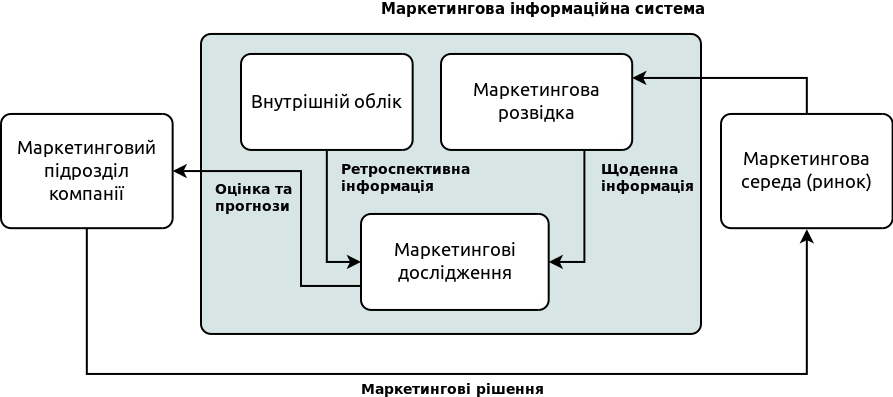
\includegraphics[width=6in]{images/mis_structure.png}
\caption{Структура МІС}
\label{fig:mis_structure}
\end{stdfigure}
 
Маркетингова інформаційна система складається з трьох частин (див. рис. \ref{fig:mis_structure}): 
\begin{itemize}
\item Внутрішній облік.
\item Маркетингові дослідження
\item Маркетингова розвідка
\end{itemize}
% Дати визначення (із посиланням на 14-те видання)
% Вставити зображення зі схемою.
% Надати опис усім трьом частинам, остання та найдетальніша: розвідка.
% TODO: що це таке, навіщо воно потрібно, складові частини та їх призначення, 4Р


\subsubsection{Маркетингова розвідка}
% TODO: Що то, нащо треба, як це робиться (моделювання, дослідження, etc), огляд наявних систем

\subsubsection{Бізнес-ігри}
% TODO: що таке бізнес-ігри, навіщо вони потрібні і як реалізються

\subsection{Постановка задачі}
\subsubsection{Моделювання маркетингового каналу}
%TODO: що таке концепція маркетингового каналу, основні момент структури та керування каналом.
% TODO: постановка задачі моделювання ()

\subsubsection{Вимоги до програмного забезпечення}